\subsection*{Teil C: Vierecke (25 Minuten)}

\begin{enumerate}[label=\arabic*.,resume]

    \item \textbf{Vierecke unterscheiden:}

    Ordne die Eigenschaften den Vierecken zu:

    \begin{center}
        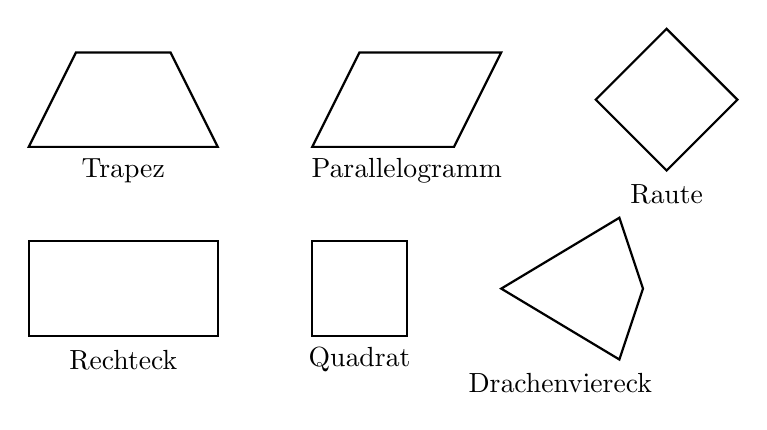
\begin{tikzpicture}[scale=0.6]
            % Trapez
            \draw[thick] (0,0) -- (4,0) -- (3,2) -- (1,2) -- cycle;
            \node at (2,-0.5) {Trapez};

            % Parallelogramm  
            \begin{scope}[xshift=6cm]
                \draw[thick] (0,0) -- (3,0) -- (4,2) -- (1,2) -- cycle;
                \node at (2,-0.5) {Parallelogramm};
            \end{scope}

            % Raute
            \begin{scope}[xshift=12cm]
                \draw[thick] (0,1) -- (1.5,2.5) -- (3,1) -- (1.5,-0.5) -- cycle;
                \node at (1.5,-1) {Raute};
            \end{scope}

            % Rechteck
            \begin{scope}[yshift=-4cm]
                \draw[thick] (0,0) rectangle (4,2);
                \node at (2,-0.5) {Rechteck};
            \end{scope}

            % Quadrat
            \begin{scope}[xshift=6cm,yshift=-4cm]
                \draw[thick] (0,0) rectangle (2,2);
                \node at (1,-0.5) {Quadrat};
            \end{scope}

            % Drachenviereck
            \begin{scope}[xshift=10cm,yshift=-4cm]
                \draw[thick] (0,1) -- (2.5,2.5) -- (3,1) -- (2.5,-0.5) -- cycle;
                \node at (1.25,-1) {Drachenviereck};
            \end{scope}
        \end{tikzpicture}
    \end{center}

    Kreuze die zutreffenden Eigenschaften an:

    \begin{center}
        \small
        \begin{tabular}{|p{2.5cm}|c|c|c|c|c|c|}
            \hline
            \textbf{Eigenschaft} & \textbf{Trapez} & \textbf{Parallel.} & \textbf{Raute} & \textbf{Rechteck} & \textbf{Quadrat} & \textbf{Drachen} \\
            \hline
            Ein Paar parallele Seiten & $\square$ & $\square$ & $\square$ & $\square$ & $\square$ & $\square$ \\
            \hline
            Zwei Paar parallele Seiten & $\square$ & $\square$ & $\square$ & $\square$ & $\square$ & $\square$ \\
            \hline
            Alle Seiten gleich lang & $\square$ & $\square$ & $\square$ & $\square$ & $\square$ & $\square$ \\
            \hline
            Alle Winkel 90° & $\square$ & $\square$ & $\square$ & $\square$ & $\square$ & $\square$ \\
            \hline
            Diagonalen gleich lang & $\square$ & $\square$ & $\square$ & $\square$ & $\square$ & $\square$ \\
            \hline
            Diagonalen stehen senkrecht & $\square$ & $\square$ & $\square$ & $\square$ & $\square$ & $\square$ \\
            \hline
        \end{tabular}
    \end{center}

    \vspace{1cm}

    \item \textbf{Viereck konstruieren:}

    Konstruiere ein Parallelogramm mit $a = 7$ cm, $b = 4$ cm, $\alpha = 120°$

    \vspace{7cm}

\end{enumerate}